\documentclass[border=4pt]{standalone}
\usepackage{amsmath,amssymb,tikz-cd}
\begin{document}
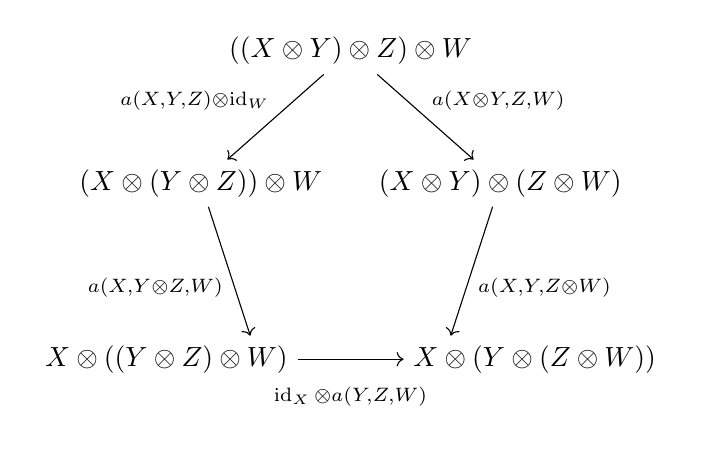
\begin{tikzpicture}[commutative diagrams/every diagram]
  \node (P0) at (90:2.3cm) {$((X \otimes Y) \otimes Z) \otimes W$};
  \node (P1) at (90+72:2cm) {$(X \otimes (Y \otimes Z)) \otimes W$};
  \node (P2) at (90+2*72:2cm) {\makebox[5ex][r]{$X \otimes ((Y \otimes Z) \otimes W)$}};
  \node (P3) at (90+3*72:2cm) {\makebox[5ex][l]{$X \otimes (Y \otimes (Z \otimes W))$}};
  \node (P4) at (90+4*72:2cm) {$(X \otimes Y) \otimes (Z \otimes W)$};
  \path[commutative diagrams/.cd, every arrow, every label]
    (P0) edge node[swap] {$a(X,Y,Z) \otimes \operatorname{id}_W$} (P1)
    (P1) edge node[swap] {$a(X, Y \otimes Z, W)$} (P2)
    (P2) edge node[swap, inner sep=1em] {$\operatorname{id}_X \otimes a(Y,Z,W)$} (P3)
    (P4) edge node {$a(X, Y, Z \otimes W)$} (P3)
    (P0) edge node {$a(X \otimes Y, Z, W)$} (P4);
  % The two makebox labels extend beyond their node widths; preserve them in the crop.
  \path (-4.1,0) (4.1,0);
\end{tikzpicture}
\end{document}
